\documentclass[10pt]{article} % Font size - 10pt, 11pt or 12pt

\usepackage[hmargin=1.25cm, vmargin=1.5cm]{geometry} % Document margins

\usepackage{graphicx}
\usepackage{amsmath}
\usepackage{marvosym} % Required for symbols in the colored box
\usepackage{ifsym} % Required for symbols in the colored box

\usepackage[usenames,dvipsnames]{xcolor} % Allows the definition of hex colors

% Fonts and tweaks for XeLaTeX
\usepackage{fontspec,xltxtra,xunicode}
\defaultfontfeatures{Mapping=tex-text}
%\setmonofont[Scale=MatchLowercase]{Andale Mono}

% Colors for links, text and headings
\usepackage{hyperref}
\definecolor{linkcolor}{HTML}{506266} % Blue-gray color for links
\definecolor{shade}{HTML}{F5DD9D} % Peach color for the contact information box
\definecolor{text1}{HTML}{2b2b2b} % Main document font color, off-black
\definecolor{headings}{HTML}{701112} % Dark red color for headings
% Other color palettes: shade=B9D7D9 and linkcolor=A40000; shade=D4D7FE and linkcolor=FF0080

\hypersetup{colorlinks,breaklinks, urlcolor=linkcolor, linkcolor=linkcolor} % Set up links and colors

\usepackage{fancyhdr}
\pagestyle{fancy}
\fancyhf{}
% Headers and footers can be added with the \lhead{} \rhead{} \lfoot{} \rfoot{} commands
% Example footer:
%\rfoot{\color{headings} {\sffamily Last update: \today}. Typeset with Xe\LaTeX}

\renewcommand{\headrulewidth}{0pt} % Get rid of the default rule in the header

\usepackage{titlesec} % Allows creating custom \section's

% Format of the section titles
\titleformat{\section}{\color{headings}
\scshape\Large\raggedright}{}{0em}{}[\color{black}\titlerule]

\title{Classical Mechanics Assignment Two}
\author{Elliott Capek}
\titlespacing{\section}{0pt}{0pt}{5pt} % Spacing around titles

\begin{document}

\maketitle{}

\section{Problem One}
\textbf{Consider  a  ball  that  moves  vertically  under  the  influences  of  both  gravity  and  air resistance.  For  the  purposes  of  this  problem,  take  vertically  upward  as  the  positive direction. (For instance, the gravitational force on the ball would be expressed as -mg in this case.) For each equation of motion below, determine whether that equation applies 
to (i) a situation in which the ball moves upward, (ii) a situation in which the ball moves 
downward, (iii) either of these, or (iv) neither of these. Explain your reasoning for each 
case. c is a positive constant. Justify each answer, no need  to add a  final paragraph of 
comment for the whole problem.} \\ \\

\begin{equation}
  m\frac{dv}{dt} = -mg + cv\\
\end{equation}
This motion equation corresponds to case (iii), either upwards or downwards motion. $\frac{dv}{dt}$ is positive when $cv > mg$, and negative when $cv < mg$. This means that in the case that v is positive and $cv$ has a larger magnitude than the downward acceleration $mg$, the acceleration will be positive and make velocity more positive, leading to upwards motion. When $cv$ is less than the magnitude of $mg$, gravity is either overcoming an upwards force or reinforcing a downward force and accelerating the ball downward.\\

\begin{equation}
  m\frac{dv}{dt} = -mg - cv\\
\end{equation}
This situation corresponds to (ii), downwards motion. When velocity is positive, it feels downward acceleration. When velocity is negative, assuming air drag is small compared to gravity, the object will travel downwards until it reaches terminal velocity.

\begin{equation}
  m\frac{dv}{dt} = -mg + cv^2\\
\end{equation}
This situation corresponds to either upward or downward motion. If $\sqrt{\frac{mg}{c}} < v$, then the object will constantly feel upward motion. If $\sqrt{\frac{mg}{c}} > v$, then the object will at first feel deceleration until v is so negative that $\sqrt{\frac{mg}{c}} < v$, at which point it will begin to accelerate until this is no longer true. It will oscillate around the negative v where $\sqrt{\frac{mg}{c}} > v$ indefinitely.

\begin{equation}
  m\frac{dv}{dt} = -mg - cv^2\\
\end{equation}
This situation corresponds to downward motion. $-cv^2$ will always be negative, and so the acceleration will always be downwards.\\

\vspace{1 cm}

\section{Problem Two}
\textbf{Express  the  terminal  velocity  of  objects  falling  vertically  in  air  and  subject to the following (fictitious) drag  forces (no need to add a  final paragraph of comment  for the whole problem):} \\ \\

a.)\\
Here we treat $\hat{v}$ as a unit vector which always points in the direction of velocity, in this case downwards.\\

\begin{align}
  \vec{F}_{drag} &= -\alpha\log(v)\hat{v}\\
  \frac{dv}{dt} &= -mg + \vec{F}_{drag}\\
  \frac{dv}{dt} &= -mg + \alpha\log(v)\\  
  \frac{dv}{dt} &= -mg + \alpha\log(v_{term}) = 0\\
  \frac{mg}{\alpha} &= \log(v_{term})\\
  \frac{mg}{\alpha} &= \log(v_{term})\\
  v_{term} &= e^{\frac{mg}{\alpha}}\\
\end{align}

This solution makes sense. It has positive sign, which makes sense, since positive sign corresponds to downward motion. Alpha is inversely proportional to terminal velocity, and mass is proportional.

b.)
\begin{align}
  \vec{F}_{drag} &= -\alpha v^3\vec{v}\\
  \vec{F}_{drag} &= -\alpha v^4\hat{v}\\  
  \frac{dv}{dt} &= -mg + \vec{F}_{drag}\\
  \frac{dv}{dt} &= -mg -\alpha v^4\hat{v}\\
  \frac{dv}{dt} &= -mg +\alpha v_{term}^4 = 0\\
  \alpha v_{term}^4 &= mg\\
  v_{term}^4 &= \frac{mg}{\alpha}\\
  v_{term} &= \sqrt[4]{\frac{mg}{\alpha}}\\
\end{align}

This solution makes sense. Terminal velocity is proportional to mass and inversely proportional to alpha, as expected. For this particular system, where force is highly velocity-dependent, the terminal velocity grows a lot slower than in the above case, where force is less strongly velocity-dependent.

\vspace{1 cm}       

\section{Problem Three}
\textbf{Consider a softball of diameter 10cm and mass 200g and one of Millikan’s oil droplets 
with  diameter  1µm  and  mass  1pg.  They  are  both subject  to  air  drag  of  equation
$\vec{F}_{drag} = −\beta D\vec{v} −\gamma D^2v\vec{v}$, with $\beta = 1.6 \times 10^{−4}$ and $\gamma = 0.25$ (SI units).} \\ \\

a. For  the  ball  and  the  droplet,  find  the  velocity  range  for  which  the  linear  (viscous) term of the drag force dominates and the one for which the quadratic (momentum) term dominates.\\

\begin{align}
  F_{vis} &> F_{mom}\\
  -\beta D\vec{v_{vis}} &> -\gamma D^2v_{vis}\vec{v}_{vis}\\
  \beta D\vec{v_{vis}} &< \gamma D^2v_{vis}\vec{v}_{vis}\\
  \beta D\vec{v_{vis}} &< \gamma D^2v_{vis}\vec{v}_{vis}\\
  \beta v_{vis} &< \gamma Dv^2_{vis}\\
  \frac{\beta}{\gamma D} &< v_{vis}\\
  \frac{\beta}{\gamma D} &< v_{vis}\\
\end{align}
Therefore, $\frac{\beta}{\gamma D}  > v_{mom}$.

Ball:
\begin{align}
  \frac{\beta}{\gamma D} < v_{vis}\\
  \frac{1.6*10^{-4}}{0.25*0.1} < v_{vis}\\
  0.0064 \frac{m}{s} < v_{vis}
\end{align}

Oil droplet:
\begin{align}
  \frac{\beta}{\gamma D} < v_{vis}\\
  \frac{1.6*10^{-4}}{0.25*10^{-6}} < v_{vis}\\
  640 \frac{m}{s} < v_{vis}
\end{align}

b. Calculate the terminal velocity of the ball and of the droplets when they are falling vertically.\\

We let $\vec{v}$ point downward, and expect positive velocities.\\

\begin{align}
  \frac{dv}{dt} &= -mg −\beta D\vec{v} −\gamma D^2v\vec{v}\\
  0 &= -mg + \beta Dv_{term} +\gamma D^2v^2_{term}\\
  0 &= \gamma D^2v^2_{term} + \beta Dv_{term} - mg\\
  v_{term} &= \frac{-\beta D \pm \sqrt{\beta^2 D^2 + 4\gamma D^2mg}}{2\gamma D^2}\\
\end{align}

Ball:
\begin{align}
  v_{term} &= \frac{-\beta D \pm \sqrt{\beta^2 D^2 - 4\gamma D^2mg}}{2\gamma D^2}\\
  v_{term} &= \frac{-1.6*10^{-4}*0.1 + \sqrt{1.6^2*10^{-8}*0.1^2 + 4*0.25*0.1^2*0.2*9.8}}{2*0.25*0.1^2}\\
  &= 27.99 \frac{m}{s}\\
\end{align}

Oil droplet:
\begin{align}
  v_{term} &= \frac{-\beta D \pm \sqrt{\beta^2 D^2 - 4\gamma D^2mg}}{2\gamma D^2}\\
  v_{term} &= \frac{-1.6*10^{-4}*10^{-6} + \sqrt{1.6^2*10^{-8}*10^{-12} + 4*0.25*10^{-12}*10^{-15}*9.8}}{2*0.25*10^{-12}}\\
  = 6.1*10^{-5} \frac{m}{s}\\
\end{align}

c. Reflect on your result. What term of the drag force is dominant  for the  free-falling softball? What term is dominant for the oil droplet?\\

The ball's terminal velocity is about 28 meters per second, which means quadratic drag is the dominating force. The oil droplet's terminal velocity is well below 640 meters per second, so it is under almost entirely linear drag. In fact, oil droplets never feel momentum/quadratic drag.\\

This problem was cool because it showed that some objects never really feel quadratic drag. Oil drops, which have very low radius, feel very little quadratic drag. Basically all objects on the size scale of an oil-drop or smaller feel mostly viscous drag from the air they move. This problem also reinforced how to calculate terminal velocity. I also had to spend some time thinking about how to deal with the coordinate system and velocity vectors and what direction they point in. I decided to make them point down, and this made the sign of the drag forces upwards. \\

\vspace{1 cm}       

\section{Problem Four}
\textbf{When a cyclist comes to a stop, without using the brakes, she is subject to two forces: the quadratic force of air resistance  $F_{air} = −cv^22$ and a constant friction force  $F_f$.} \\ \\

a. Write and solve the equation of motion for the velocity as a function of time while the cyclist is coasting to a halt.\\

\begin{align}
  m\frac{dv}{dt} = -F_f - cv^2\\
  m\frac{dv}{-F_f - cv^2} = dt\\
  \int_{v0}^v m\frac{dv}{-F_f - cv^2} = \int dt\\
  \int_{v0}^v \frac{mdv}{F_f + cv^2} = -t\\
  \frac{m*\tan^{-1}(\frac{\sqrt{c}v}{\sqrt{F}})}{\sqrt{cF}} - \frac{m*\tan^{-1}(\frac{\sqrt{c}v_0}{\sqrt{F}})}{\sqrt{cF}} = -t\\
  \tan^{-1}(\frac{\sqrt{c}v}{\sqrt{F}}) - \tan^{-1}(\frac{\sqrt{c}v_0}{\sqrt{F}}) = \frac{-t\sqrt{cF}}{m}\\
  \tan^{-1}(\frac{\sqrt{c}v}{\sqrt{F}}) = \frac{-t\sqrt{cF}}{m} + \tan^{-1}(\frac{\sqrt{c}v_0}{\sqrt{F}})\\  
  \tan(\frac{-t\sqrt{cF}}{m} + \tan^{-1}(\frac{\sqrt{c}v_0}{\sqrt{F}})) = \frac{\sqrt{c}v}{\sqrt{F}}\\
  \sqrt{\frac{F}{c}}\tan(\frac{-t\sqrt{cF}}{m} + \tan^{-1}(\frac{\sqrt{c}v_0}{\sqrt{F}})) = v(t)\\    
\end{align}

b. Plot  a  graph  of  the  result  for  a  cyclist  plus  bike  mass  of  80kg,  an  initial  velocity 20m/s, a quadratic drag coefficient  c = 0.2 (in SI units) and a  friction  force of 3 N.\\

\begin{figure}[h!]
  \caption{Plot of cyclist velocity over time.}
  \centering
    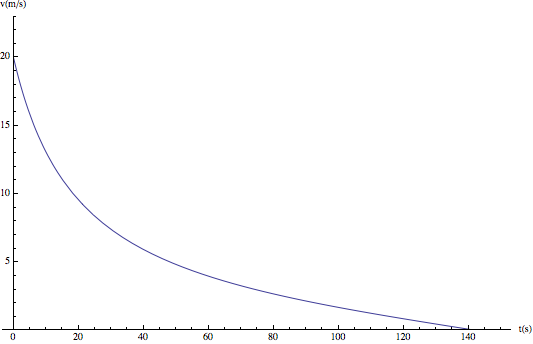
\includegraphics[width=0.7\textwidth]{images/cyclist_velocity_m1.png}
\end{figure}

Answer the following graphically:\\
- How long will it take the cyclist to slow down to 15 m/s?\\

By examining the graph, we can see that it takes roughly ten seconds for the cyclist to slow from 20 m/s to 15 m/s.\\

- How long to slow from 10m/s to 5m/s?\\

Also by inspection of teh graph, we can see that it takes roughly 25 seconds to slow from 10m/s to 5m/s.\\

- How long does it take for a complete stop (from the initial velocity to 0m/s)?\\
It takes roughly 140 seconds to reach a complete stop, starting at 20m/s.\\

This was a harder problem, but also intersting. We had to use the basic technique of physics, finding a differential equation to model a system and solving for velocity (or usually position), then use a computer to plot this solution, since it is difficult to interpret otherwise. I learned that from very simple initial forces (a constant force and a velocity squared force, both opposing motion), the equation for velocity can become complex (this one involved a tangent function).

\section{Problem Five}

\textbf{A particle is fired vertically upward in a constant gravitational field with an initial speed $v_0$.  Show  that  if  there  is  a  retarding  force  proportional  to  the  square  of  the instantaneous speed, the speed of the particle when it returns to the initial position is:}

$$ v = \frac{v_ov_{term}}{\sqrt{v_0^2+v^2_{term}}}  $$

\textbf{where $v_{term}$ is the terminal velocity.}

We need to solve the following differential equation:\\

When going up:\\
\begin{align}
  m\frac{dv}{dt} = -mg - cv^2\\
  m\frac{dv}{dy}\frac{dy}{dt} = -mg - cv^2\\
  m\frac{dv}{dy}v = -mg - cv^2\\
  m\frac{dv}{-mg - cv^2}v = dy\\
  \int_{v_0}^0 m\frac{dv}{-mg - cv^2}v = \int dy\\
  \int_{v_0}^0 m\frac{mv}{-mg - cv^2}dv = y_{max}\\
  \int_{v_0^2}^0 \frac{mv}{-mg - cu}\frac{du}{2v} = y_{max}\\
  \frac{1}{2} \int_{v_0^2}^0 \frac{m}{-mg - cu} du = y_{max}\\
  \frac{m \log(cv_0^2 + gm)}{2c} - \frac{m \log(gm)}{2c} = y_{max}\\
  \frac{m}{2c} \log(\frac{cv_0^2 + gm}{gm}) = y_{max}\\  
\end{align}

When falling back down:\\
\begin{align}
  m\frac{dv}{dt} = -mg + cv^2\\
  m\frac{dv}{dy}\frac{dy}{dt} = -mg + cv^2\\
  m\frac{dv}{dy}v = -mg + cv^2\\
  m\frac{dv}{-mg + cv^2}v = dy\\
  \int_{0}^{vf} m\frac{dv}{-mg + cv^2}v = \int dy\\
  \int_{0}^{vf} m\frac{mv}{-mg + cv^2}dv = -y_{max}\\
  \int_{0}^{vf} \frac{mv}{-mg + cu}\frac{du}{2v} = -y_{max}\\
  \frac{1}{2} \int_{0}^{vf} \frac{m}{-mg + cu} du = -y_{max}\\
  \frac{m \log(cv_f^2 - gm)}{2c} - \frac{m \log(-gm)}{2c} = -y_{max}\\
  \frac{m}{2c} (\log(cv_f^2 - gm) - \log(-gm)) = -y_{max}\\
  \frac{m}{2c} \log(\frac{cv_f^2 - gm}{-gm}) = -y_{max}\\
  \frac{m}{2c} \log(\frac{gm - cv_f^2}{gm}) = y_{max}\\
\end{align}

We now find $v_{term}$:

\begin{align}
  m\frac{dv}{dt} = -mg + cv^2 = 0\\
  -mg + cv_{term}^2 = 0\\
  cv_{term}^2 = mg\\
  v_{term} = \sqrt{\frac{mg}{c}}\\
\end{align}

We now have two expressions for $y_{max}$. We set them equal and see what we get:

\begin{align}
  \frac{m}{2c} \log(\frac{gm}{cv_0^2 + gm}) = \frac{m}{2c} \log(\frac{gm - cv_f^2}{gm})\\
  \frac{gm}{cv_0^2 + gm} = \frac{gm - cv_f^2}{gm}\\
  \frac{(gm)^2}{cv_0^2 + gm} = gm - cv_f^2\\
  cv_f^2 = gm - \frac{(gm)^2}{cv_0^2 + gm}\\
  v_f^2 = \frac{gm}{c} - \frac{(gm)^2}{c^2v_0^2 + cgm}\\
  v_f^2 = v_{term}^2 - \frac{v_{term}^4}{v_0^2 + v_{term}^2}\\
  v_f^2 = \frac{v_{term}^2(v_0^2 + v_{term}^2) - v_{term}^4}{v_0^2 + v_{term}^2}\\
  v_f^2 = \frac{v_{term}^2v_0^2}{v_0^2 + v_{term}^2}\\      
\end{align}

This was a really interesting problem in that it had us do a fairly lengthy derivation of something. We had to apply lots of different knowledge - tricky integration, terminal velocity calculation and logarithm manipulation. It was really intersting to see how all the little parts fit together. This was probably the hardest part of the problem set in that it was really hard to get the correct answer, but it was a fun problem and a good test of math skills.\\

\end{document}
